\documentclass[12pt]{article}

\usepackage[T1]{fontenc}
\usepackage[utf8]{inputenc}
\usepackage[spanish, mexico]{babel}
\usepackage[autostyle]{csquotes}
\usepackage{fancyvrb}
\usepackage{multicol}
\usepackage{graphicx}
\usepackage{enumitem}

\usepackage{array}
\setlength{\tabcolsep}{1em}
\renewcommand{\arraystretch}{1.5}

\usepackage[T1]{fontenc}

\usepackage[margin=1in,marginparwidth=3in]{geometry}

\usepackage{fancyhdr}
\pagestyle{fancy}
\fancyhf{}
\fancyhead[L]{\leftmark}
\fancyfoot[C]{\thepage}
\setlength{\headheight}{14.61858pt}

\usepackage{mathtools}
\usepackage{amssymb}
\usepackage{amsthm}
\usepackage[backend=bibtex, style=ieee]{biblatex}
\addbibresource{fuentes.bib}

\usepackage{hyperref}
\hypersetup{
    colorlinks=true,
    pdftitle={Conceptos básicos de LaTeX},
}

\addtolength{\topmargin}{-0.1638pt}

\newtheorem{theorem}{Teorema}

\author{Francisco Galindo}
\title{Conceptos básicos}

\begin{document}

\maketitle
\tableofcontents

\section{Objetivos de estas sesiones}

El objetivo de las primeras sesiones de este curso es que ustedes puedan, ya
sea por gusto o por necesidad, crear un documento en \LaTeX{}, agregando la
gran mayoría de los elementos a los que ya están acostumbrados en otros
sistemas de procesamiento de textos, como la justificación de texto, adición de
imágenes y de tablas. Además, conocerán algunos de los elementos que hacen
único a \LaTeX{} con respecto a los sistemas más populales, como su composición
de ecuaciones y su manejo de bibliografía.

\section{¿Qué son \TeX{} y \LaTeX?}

\TeX{} es un \emph{lenguaje de
marcado}\footnote{\url{https://en.wikipedia.org/wiki/Markup_language}} creado
por Donald Knuth para componer documentos con un aspecto consistente y
atractivo. Knuth estaba inconforme con la calidad cada vez menor en la
tipografía de su libro \textit{El arte de programar computadoras}. En un año
sabático que se tomó (1978) inició el desarrollo del lenguaje, que se consideró
\textit{feature-complete}\footnote{\url{https://en.wikipedia.org/wiki/Software_release_life_cycle\#Feature-complete}}
en 1985 y desde entonces las únicas actualizaciones hechas son correcciones de
\textit{bugs}.

\LaTeX{} es un sistema de preparación de documentos \cite{latex:1} creado por
Leslie Lamport en 1984. Suele usarse para publicaciones técnicas o científicas,
pero puede usarse para preparar casi cualquier tipo de documento. Se trata de
un grupo de comandos de \TeX{} cuyo propósito es simplificar el uso de \TeX{}.
El desarrollo de \LaTeX{} se basa en la idea de que es mejor separar las tareas
de diseño de aquellas de escritura.

\subsection{¿Qué gano al aprender \LaTeX?}

La forma de trabajar en \LaTeX{} es bastante diferente a comparación de
sistemas de procesamiento de textos como \textit{Microsoft Word},
\textit{Google Docs}, o \textit{Libre Office Writer}. En estos últimos, la
edición del texto se hace en el mismo lugar en el que se hacen las ediciones de
estilo. Es decir, el contenido del documento se edita en el mismo lugar y al
mismo tiempo que su formato (fuente, tamaño de letra, justificación, etc.). 

\LaTeX{}, por su parte, trabaja ``editando código'' de manera similar a lo que
se haría al utilizar un lenguaje de programación u otro lenguaje de marcado
como HTML. El escritor crea un archivo de texto con todo el contenido del
documento y los comandos correspondientes de manera estructurada de acuerdo con
su significado e importancia, y mediante un compilador, este archivo de texto
(archivo fuente) se convierte a un formato que pueda ser leído por el público,
(por ejemplo, formato PDF). El diseño estético del documento generalmente se
hace por separado, muchas veces por otra persona.

Este cambio de paradigma trae consigo una serie de ventajas y de desventajas.
De primeras, se pierden algunas cosas:
\begin{itemize}
    \item No necesariamente puedes ver la versión final del documento mientras
        lo editas.
    \item Tienes que aprender todos los comandos necesarios para escribir tu
        documento.
    \item Muchas veces es difícil que el documento se vea \emph{exactamente}
        como deseas.
\end{itemize}

Sin embargo, la filosofía de uso de \LaTeX{} brinda muchas ventajas:
\begin{itemize}
    \item Se puede editar el contenido del documento con cualquier editor de
        texto. No estás limitado a utilizar cierto editor como es el caso con
        los programas.
    \item Suponiendo que tú o alguien más ya definió el estilo del documento,
        puedes enfocarte enteramente en la creación de la estructura conceptual
        y contenidos del documento.
    \item La generación de elementos repetitivos como índices, notas al pie, y
        referencias se hace de manera automática.
    \item Debido a que el archivo fuente del documento es texto plano, puede
        ser compartido, entendido y modificado para las necesidades de otras
        personas. Es más difícil saber cómo alguien hizo que un documento de
        \textit{Word} se viera de cierta manera que en \LaTeX{}.
    \item Elementos como ecuaciones, tablas, y figuras pueden ser generados de
        manera programática con cualquier otro lenguaje.
    \item Puede utilizarse cualquier otro lenguaje de marcado para crear un
        documento, que sea más sencillo de usar, y posteriormente convertirlo a
        un documento de \LaTeX{} a partir del cuál se pueda generar un PDF o
        archivo similar.
\end{itemize}


\section{Sintaxis básica}

Un documento de \LaTeX{} es un archivo en texto plano que puede ser escrito en
cualquier editor de texto. Contienen el texto del documento así como los
comandos de \LaTeX{} necesarios para componer el texto. Un ejemplo muy básico
se ve así:

\begin{Verbatim}[frame=single]
    \documentclass{article}

    \title{Mi primer documento}
    \author{Francisco Galindo}
    \date{2024}

    \begin{document}
    \maketitle
    ¡Hola, mundo!
    \end{document}
\end{Verbatim}

\begin{itemize}
    \item Este documento es un artículo.
    \item Su título es ``Mi primer documento''.
    \item Su autor es Francisco Galindo.
    \item Fue escrito en 2024.
    \item El documento consiste de un título seguido del texto ``¡Hola, mundo!''.

\end{itemize}

Se obtiene el siguiente resultado:

\begin{center}
\noindent\fbox{%
    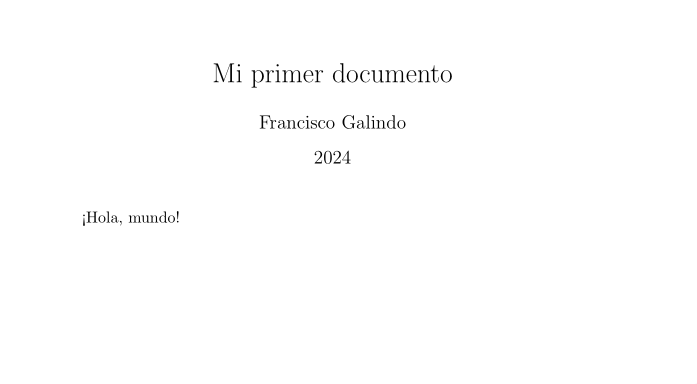
\includegraphics[width=\textwidth - 8\fboxsep]{img/primer-docu}
}
\end{center}

\subsection{Escribiendo texto}

\subsubsection{Espacios en blanco}

Cualquier grupo de espacios en blanco se verá, en el 

\subsubsection{Secciones, subsecciones, etc.}

Para jerarquizar el contenido del documento, existen los comandos \\
\verb|\section|, \verb|\subsection|, \verb|\subsubsection|, \verb|\paragraph|,
y \verb|\subparagraph|:

\begin{Verbatim}[frame=single]
    \section{Una sección}

    Consectetur laboriosam nulla libero quisquam quos..

    \subsection{Una subsección}

    Consectetur magnam esse illum nobis enim magni?

    \subsubsection{Una subsubsección}

    Elit eius quas eveniet delectus doloremque.

    \paragraph{Un párrafo}: Amet alias doloribus sequi
    Natus repellat.

    \subparagraph{Subpárrafo}: Adipisicing amet Earum fugit at
    qui illum praesentium?
\end{Verbatim}

\subsubsection{\textit{Itálicas} y \textbf{negritas}}


\subsection{Comandos}

Un comando es un aglomerado de operaciones que \LaTeX{} ejecutará al momento de
que el comando sea escrito. La mayoría de los comandos en \LaTeX{} son una
palabra con una anti-diagonal (\verb|\|) al principio. Un comando puede llegar
a necesitar un argumento, que es escrito entre llaves (\verb|{}|) al final del
nombre del comando. Algunos comandos pueden aceptar parámetros opcionales, que
son añadidos después del nombre del comando y antes del argumento del mismo
dentro de corchetes (\verb|[]|) y separados entre comas (,). Una llamada a un
comando se ve así:
    

\begin{Verbatim}[frame=single]
    \nombredelcomando[parámetro1, parámetro2, ...]{argumento}
\end{Verbatim}

\subsection{Ambientes}

Un ambiente funciona de manera similar a un comando común, pero generalmente
tienen un efecto sobre una parte más larga del documento, como un párrafo
entero en lugar de una sola oración. Su sintaxis de uso es:

\begin{Verbatim}[frame=single]
    \begin{ambiente}
        Texto afectado por el ambiente...
    \end{ambiente}
\end{Verbatim}

\hypertarget{groups}{}
\subsection{Grupos}

Algunos comandos funcionan a manera de \textit{switch}, es decir, que afectan
al resto del documento después de haber sido ejecutados:

\begin{Verbatim}[frame=single]
    \begin{document}
        Este texto es normal

        \itshape 

        Este texto está en itálicas.
        ...
        Todo el documento está en itálicas ahora.
        ...
    \end{document}
\end{Verbatim}

Para limitar el ámbito de influencia (\textit{scope}) de este tipo de comandos,
se hace uso de grupos. Un grupo puede crearse al encerrar la parte del
documento que se quiere afectar (incluyendo al \textit{switch}) en llaves
(\verb|{}|). También pueden utilizarse los comandos \verb|\bgroup| y
\verb|\egroup| para iniciar y terminar un grupo, respectivamente.

\begin{Verbatim}[frame=single]
    \begin{document}
    Texto normal {\itshape texto en itálica} más texto normal.

    Texto normal \bgroup \itsahpe texto itálica \egroup{} texto normal.
    \end{document}
\end{Verbatim}

\subsection{Comentarios}

El símbolo \verb|%| es utilizado para denotar un comentario. Cuando \LaTeX{}
está procesando un documento y se encuentra con un \verb|%|, ignora el resto
de la línea. De esta manera, un comentario se puede utilizar para escribir
notas en el archivo fuente que no serán visibles en la versión final del
documento.

\subsection{Clases y paquetes}

Una clase define cómo se ve, a groso modo el documento que estás escribiendo.
Se trata de un grupo de comandos que se ejecutan para darle el estilo deseado
al documento. Se seleccionan con el comando \verb|\documentclass|. Se hablará
más de clases de documentos en próximas sesiones.

Un paquete es similar a una biblioteca en un lenguaje de programación. Incluyen
una serie de características adicionales que puedes utilizar en tu documento,
como el uso de colores, adición de imágenes o inclusión de nuevos comandos y
ambientes.


\section{Agregando contenido al documento}

\subsection{Escribiendo matemáticas}

\subsubsection{Ambientes para matemáticas}

Al momento de escribir expresiones matemáticas, \LaTeX{} necesita saber dónde
empiezan y terminan las mismas. Existen dos ambientes distintos para presentar
texto matemático:

\begin{itemize}
    \item \emph{inline}: las fórmulas aparecen como parte de un párrafo de
        texto. Un ejemplo es este: \((a-b)(a+b) = a^2-b^2\).
    \item \emph{display}: se utiliza para escribir expresiones que no son parte
        de un párrafo, es decir, que aparecen en una línea por sí mismas. Por
        ejemplo:
        \[
            (a-b)(a+b) = a^2 - b^2.
        \]
\end{itemize}

Los ambientes correspondientes a ambos tipos de expresiones se pueden utilizar
así:

\begin{Verbatim}[frame=single]
    \begin{math} % modo inline
        ...
    \end{math}

    \begin{displaymath} % modo display
        ...
    \end{displaymath}
\end{Verbatim}

Como un documento puede contener muchas (¡muchas!) ecuaciones, \LaTeX{} tiene
``abreviaciones'' para entrar en estos modos, \verb+\(...\)+ para el modo
\textit{inline} y \verb+\[...\]+ para \textit{display}. Por ejemplo, este
pedazo de código tiene el siguiente resultado:

\begin{Verbatim}[frame=single]
    Una ecuación en modo \textit{inline} enmedio de una oración:
    \(x = \frac{-b \pm \sqrt{b^2 - 4ac}}{2a}\).

    Esta es la misma ecuación en modo \textit{display}:
    \[x = \frac{-b \pm \sqrt{b^2 - 4ac}}{2a}.\]
\end{Verbatim}

\noindent\fbox{%
    \parbox{\linewidth - 2.3\fboxsep}{%
        Una ecuación en modo \textit{inline} enmedio de una oración:
        \(x = \frac{-b \pm \sqrt{b^2 - 4ac}}{2a}\).

        Esta es la misma ecuación en modo \textit{display}:
        \[x = \frac{-b \pm \sqrt{b^2 - 4ac}}{2a}.\]
    }%
}

\subsubsection{Símbolos matemáticos y }

\subsubsection{Sumas, integrales y límites}

El símbolo de una integral puede escribirse con el siguiente comando:\\
\verb+\int_{inf}{sup}+, donde \texttt{inf} y \texttt{sup} son los límites de
integración. Pueden escribirse integrales múltiples, así como integrales cerradas como esta:
\[
    \oint_{\gamma} F \cdot \,dr = \iint_S \nabla \times F \cdot \,dS.
\]


\begin{table}
    \begin{center}
        {\renewcommand{\arraystretch}{1.3}
            \begin{tabular}{c | c | c}
                \textbf{Código} & \textbf{Res. \textit{inline}} & \textbf{Res. \textit{display}}\\
                \hline
                \verb#\int f(x)\,dx# & \(\int f(x) \,dx\) &  \( \displaystyle \int f(x) \,dx\) \\
                \hline
                \verb+\int_{a}^{b} f(x)\,dx+ & \(\int_{a}^{b} f(x) \,dx\) &  \( \displaystyle \int_{a}^{b} f(x) \,dx\) \\
                \hline
                \verb+\iint_{S} f(x,y)\,dA+ & \(\iint_{S} f(x,y) \,dA\) &  \( \displaystyle \iint_{S} f(x,y) \,dA\) \\
                \hline
                \verb+\iiint_E f(x,y,z)\,dV+ & \(\iiint_E f(x,y,z) \,dV\) &  \( \displaystyle \iiint_E f(x,y,z) \,dV\) \\
                \hline
                \verb+\oint_{\gamma} f(z)\,dz+ & \(\oint_{\gamma} f(z)\,dz\) &  \( \displaystyle \oint_{\gamma} f(z)\,dz\) \\
                \hline
                \verb+\idotsint f(x_1, \dots, x_k)+ & \( \idotsint f(x_1, \dots, x_k) \) & \( \displaystyle \idotsint f(x_1, \dots, x_k) \) \\
                \hline
            \end{tabular}
        }
    \end{center}
    \caption{Ejemplos de varios tipos de integrales con ayuda del paquete}
\end{table}

\subsubsection{Matrices}

\[
    \iint_V \mu(u,v) \,du\,dv
\]

\begin{theorem}
    El valor de \(\int_{-\infty}^{\infty} e^{-x^2} \,dx\) es
    \[
        \int_{\infty}^{\infty} e^{-x^2} \,dx = \sqrt{\pi}.
    \]
\end{theorem}

\begin{proof}
    \begin{align*}
        \left( \int_{-\infty}^{\infty} e^{-x^2} \,dx\right)^2 
        &=
        \left( \int_{-\infty}^{\infty} e^{-x^2} \,dx \right)
        \left( \int_{-\infty}^{\infty} e^{-y^2} \,dy \right) && \text{por (\ref{eqn:eigen-1})} \\
        %
                                                             &= \int_{-\infty}^{\infty} \int_{-\infty}^{\infty} e^{-x^2} e^{-y^2} \,dx\,dy\\
                                                             &= \int_{-\infty}^{\infty} \int_{-\infty}^{\infty} e^{-(x^2 + y^2)} \,dx\,dy\\
                                                             &= \int_{0}^{2\pi} \int_{0}^{\infty} e^{-r^2} r \,dr\,d\theta\\
                                                             &= \int_{0}^{2\pi} \left[ - \frac{e^{-r^2}}{2} \right]_{r=0}^{r=\infty} \,d\theta\\
                                                             &= \int_{0}^{2\pi} \frac{1}{2} \,d\theta\\
                                                             &= \pi
    \end{align*}
\end{proof}

\begin{equation} \label{eqn:iden-euler}
    e^{i \pi} + 1 = 0
\end{equation}

El resultado obtenido en la ecuación \ref{eqn:iden-euler} es de gran
importancia en el análisis complejo.

Considere el operador lineal $A : \mathbb{R}^n \to \mathbb{R}^n $, definido por
una matriz $\mathbf{A}$ de la siguiente manera:
\[
    \mathbf{A}v = w
\]
que también puede escribirse como
\[
    \begin{pmatrix}
        a_{11} & a_{12} & \dots & a_{1n}\\
        a_{21} & a_{22} & \dots & a_{2n}\\
        \vdots & \vdots & \ddots& \vdots\\
        a_{n1} & a_{n2} & \dots & a_{nn}
    \end{pmatrix}
    \begin{pmatrix}
        v_1 \\
        v_2\\
        \vdots\\
        v_n
    \end{pmatrix}
    =
    \begin{pmatrix}
        w_1 \\
        w_2\\
        \vdots\\
        w_n
    \end{pmatrix}
    .
\]

Si se cumple que
\begin{equation} \label{eqn:eigen-1}
    \mathbf{A} v = \lambda v
\end{equation}
entonces se dice que $v$ y $\lambda$ son un \emph{eigenvector} y un
\emph{eigenvalor} de $A$, respectivamente.

La ecuación \ref{eqn:eigen-1} puede escribirse como
\[
    (\mathbf{A} - \lambda I)\,v = 0,
\]
y, resolviendo para $\lambda$, se sabe que esta ecuación sólo tiene una
solución no trivial cuando
\[
    \det(\mathbf{A} - \lambda I) = 0,
\]
que también se puede escribir como
\[
    \begin{vmatrix}
        a_{11} - \lambda & a_{12}           & \dots  & a_{1n}\\
        a_{21}           & a_{22} - \lambda & \dots  & a_{2n}\\
        \vdots           & \vdots           & \ddots & \vdots\\
        a_{n1}           & a_{n2}           & \dots  & a_{nn} - \lambda
    \end{vmatrix}
    = 0.
\]

% \subsection{Figuras}
%
% \subsubsection{Imágenes}
%
% \subsubsection{Tablas}

\subsection{Notas}

\subsubsection{Notas al pie}

Una nota al pie de página puede crearse con el comando \verb+\footnote+. Estas
notas son enumeradas de manera automática:

\begin{Verbatim}[frame=single]
    Aquí tengo un párrafo en el que quiero hacer una
    aclaración\footnote{Soy una nota al pie.}, aunque
    no me gustaría interrumpir el texto. Puedo crear
    varias notas al pie\footnote{Soy otra nota.}.
\end{Verbatim}

\noindent\fbox{%
    \parbox{\linewidth - 2.3\fboxsep}{%

        \begin{minipage}{\textwidth - 1em}
            Aquí tengo un párrafo en el que quiero hacer una
            aclaración\footnote{Soy una nota al pie.}, aunque
            no me gustaría interrumpir el texto. Puedo crear
            varias notas al pie\footnote{Soy otra nota.}.
        \end{minipage}
    }%
}

Si no es conveniente indicar que existe la nota y escribir el contenido de la
nota al mismo tiempo, pueden utilizarse los comandos \verb|\footnotemark| y
\verb|\footnotetext| para hacer ambas cosas en pasos separados. El siguiente
pedazo de código tiene el mismo resultado que haber utilizado el comando
\verb|\footnote| directamente.

\begin{Verbatim}[frame=single]
    Sé que va a haber una nota aquí\footnotemark{}. Aut animi
    quasi aliquam cumque magnam autem Impedit deserunt quia
    nulla voluptates similique similique consectetur,
    dignissimos! Provident ab?

    \footnotetext{Este es el texto de la nota.}
\end{Verbatim}

\subsubsection{Notas al margen}

El comando \verb|\marginpar{texto}| creará un párrafo en el margen de la página
a la altura en la que haya sido llamado. Por defecto, estos párrafos se colocan
``afuera'' de la página:

\begin{Verbatim}[frame=single]
    Ipsum corporis ea doloribus corrupti ullam sequi Suscipit
    omnis dolores doloremque magni optio! Et dolor obcaecati
    \marginpar{Soy una nota al margen} nesciunt ut repellat 
    Provident deleniti hic illo quam iusto maxime minima harum?
    Cum dolores? Elit corporis recusandae atque minima voluptatum
    necessitatibus Cum neque quaerat suscipit non sed! Quasi
    sapiente ratione incidunt explicabo id beatae Aliquid beatae
    corporis sapiente assumenda culpa Soluta illo nobis
    exercitationem.
\end{Verbatim}

\noindent\fbox{%
    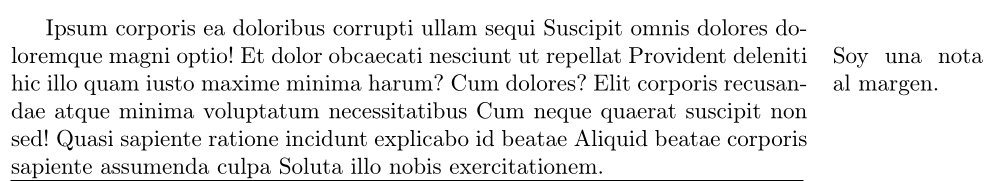
\includegraphics[width=\textwidth - 4\fboxsep]{img/margin}
}

\subsection{Enlaces}

Es deseable que, al momento de compilar un documento a algún formato de
visualización, como PDF, existan herramientas de navegación para facilitar la
vida del lector. El paquete \verb|hyperref| se encarga de gestionar la creación
de enlaces dentro del documento. Por ejemplo, simplemente al
importar\footnote{Es recomendable que este sea el último paquete en importarse,
para evitar conflictos.} el paquete, todos los elementos del documento a los
que se les haga referencia durante el documento, como figuras, ecuaciones, o
los elementos del índice, se convertirán en hipervínculos.

Se puede configuar el paquete para modificar su comportamiento com el comando \\
\verb|\hypersetup|. Por ejemplo, este documento utiliza el comando de la
siguiente manera:

\begin{Verbatim}[frame=single]
    \hypersetup{
        colorlinks=true, % Para que los enlaces tengan color

        pdftitle={Conceptos básicos de LaTeX},  % Titulo que
        % aparece en
        % lectores PDF
    }
\end{Verbatim}

Los parámetros modificables pueden encontrarse en este
\href{https://www.overleaf.com/learn/latex/Hyperlinks#Reference_guide}{enlace}.

\subsection{Agregando enlaces en el texto}

\subsubsection{Enlaces web}

Para crear un enlace para, por ejemplo, una página web puede utilizarse el
comando \verb|\url| o \verb|\href|. El primero mostrará el enlace en sí,
mientras que el segundo lo esconde para mostrar en su lugar cierto texto:

\begin{Verbatim}[frame=single]
    Puedo escribir un enlace directamente:
    \url{www.https://wikipedia.org/}.
    También puedo hacer que en su lugar aparezca una
    \href{https://wikipedia.org/}{oración}.
\end{Verbatim}

\noindent\fbox{%
    \parbox{\linewidth - 2.3\fboxsep}{%

        \begin{minipage}{\textwidth - 1em}
            Puedo escribir un enlace directamente:
            \url{www.https://wikipedia.org/}.
            También puedo hacer que en su lugar aparezca una
            \href{https://wikipedia.org/}{oración}.
        \end{minipage}
    }%
}

\subsubsection{Agregando enlaces arbitrarios}

Es posible crear enlaces que lleven a la parte del documento que se desee. Para
esto, se utilizan los comandos \verb|\hyperlink{etiqueta}{texto}| y
\verb|\hypertarget{etiqueta}{texto}|:

\begin{Verbatim}[frame=single]
    En otra parte del documento, hay una 
    \hyperlink{importante}{oración importante}.

    Esta es una oración
    \hypertarget{importante}{de gran importancia}.
\end{Verbatim}

\noindent\fbox{%
    \parbox{\linewidth - 2.3\fboxsep}{%

        \begin{minipage}{\textwidth - 1em}
            En otra parte del documento, hay una 
            \hyperlink{importante}{oración importante}.

            Esta es una oración
            \hypertarget{importante}{de gran importancia}.
        \end{minipage}
    }%
}
\section{Dándole formato al documento}

\subsection{Interlineado}

El paquete \verb|setspace| incluye los comandos necesarios para establecer
el interlineado de los párrafos, ya sea en el documento entero o en alguna
sección:
\begin{itemize}
    \item \verb|\doublespacing| para espaciado doble.
    \item \verb|\onehalfspacing| para espaciado 1.5.
    \item \verb|\singlespacing| para espaciado simple.
\end{itemize}

Estos comandos pueden usarse en el preámbulo del documento para que afecten
todo el texto, o en alguna zona local por medio de un
\hyperlink{groups}{grupo}.

\subsection{Espaciado entre párrafos}

Muchas veces, es necesario implementar disposiciones de párrafos donde los
mismos están separados por cierto espacio vertical además (o en lugar) de tener
una sangría. El paquete \verb|parskip| facilitar hacer estas configuraciones de
texto. El paquete sólo necesita ser cargado con \verb|\usepackage| para tomar
efecto. Dependiendo de las opciones (como las te la tabla \ref{tbl:parskip})
que sean enviadas al paquete, se puede modificar el espaciado entre párrafos
así como el tamaño de la sangría.

\begin{table}
    \centering
    \begin{tabular}{|c|m{2in}|}
        \hline
        \textbf{Opción} & \textbf{Descripción} \\
        \hline
        \texttt{skip} & Indica, de manera explícita, la distancia vertical entre un párrafo y otro. \\
        \hline
        \texttt{indent} & Configura la longitud de la sangría del primer renglón del párrafo. \\
        \hline
    \end{tabular}
    \label{tbl:parskip}
    \caption{Algunas de las opciones del paquete \texttt{parskip}.}
\end{table}

Un ejemplo, donde se necesita que no haya sangría, que el espacio entre
párrafos sea de \verb|1em| y con interlineado doble sería el siguiente:

\begin{Verbatim}[frame=single]
    \documentclass{article}

    % ...
    \usepackage[indent=0cm, skip=1em]{parskip}
    \usepackage{setspace}
    \doublespacing
    % ...

    \begin{document}
        Blah, blah, blah...
    \end{document}
\end{Verbatim}

\subsection{Alineación de texto}

Por defecto, \LaTeX{} justifica el texto de cada párrafo para que se vea
``parejo'', pero a veces es deseable alinear el texto de otras formas. Ya
vienen incluidos varios comandos y ambiente para alinear el texto del
documentos, pero el paquete \texttt{ragged2e} refina estos comandos para que la
separación de palabras sea más natural.

El paquete \texttt{ragged2e} incluye los siguientes comandos que funcionan a
manera de switch:

\begin{itemize}
    \item \verb|\RaggedRight| para alinear a la izquierda (el lado derecho
        queda ``accidentado'').
    \item \verb|\RaggedLeft| para alinear a la derecha.
    \item \verb|\Centering| para centrar texto.
    \item \verb|\justifying| para justificar texto.
\end{itemize}

También incluye algunos ambientes con fines similares, pero con la ventaja de
la creación implícita de grupos:

\begin{itemize}
    \item \verb|FlushLeft| para alinear a la izquierda.
    \item \verb|FlushRight| para alinear a la derecha.
    \item \verb|Center| para centrar texto.
    \item \verb|justify| para justificar texto.
\end{itemize}

%
% \subsection{Fuentes}
%
% \subsubsection{Cambiando la fuente del documento}
%
% \section{Manejo básico de bibliografía}



\nocite{*}
\printbibliography[heading=bibintoc,title={Referencias}]

\end{document}
